\documentclass[tikz,border=5pt]{standalone}
\usepackage[UTF8]{ctex}\usepackage{amsmath,amssymb}
\usetikzlibrary{arrows.meta,calc}
\definecolor{ink}{HTML}{243447}\definecolor{blue}{HTML}{2765A2}
\definecolor{green}{HTML}{3F7D5B}\definecolor{red}{HTML}{B74739}
\tikzset{body/.style={draw=ink,thick},vec/.style={draw=blue,thick,-{Latex}},guide/.style={gray!65,dashed},dim/.style={ink,{Latex}-{Latex}},line cap=round,line join=round}
\begin{document}
\begin{tikzpicture}
 \fill[blue!7](0,0)rectangle(3,1.9);
 \draw[body](6,0)--(0,0)--(0,1.9)--(6,1.9);
 \draw[body,fill=gray!25](3,0)rectangle(3.15,1.9);
 \node at(1.5,.95){$p_0,V_0,T_0$};
 \node at(4.65,.95){外界 $p_0$};
 \node[above]at(3.08,1.95){$S$};
 \node at(3,2.45){$f=p_0S/4,\quad C_V=5R/2$};
\end{tikzpicture}
\begin{tikzpicture}
 \foreach\X in{0,5.2}{\draw[body,fill=gray!15](\X+.9,0)rectangle(\X+1.1,2);}
 \draw[vec](-.5,1.5)--(.9,1.5)node[midway,above]{$p_+S$};
 \draw[red,thick,-{Latex}](2.7,1.5)--(1.1,1.5)node[midway,above]{$p_0S$};
 \draw[green,thick,-{Latex}](2.5,.5)--(1.1,.5)node[midway,below]{$f$};
 \draw[vec](.4,2.35)--(1.8,2.35)node[midway,above]{膨胀};
 \draw[vec](4.7,1.5)--(6.1,1.5)node[midway,above]{$p_-S$};
 \draw[red,thick,-{Latex}](7.9,1.5)--(6.3,1.5)node[midway,above]{$p_0S$};
 \draw[green,thick,-{Latex}](4.7,.5)--(6.1,.5)node[midway,below]{$f$};
 \draw[vec](7,2.35)--(5.6,2.35)node[midway,above]{压缩};
\end{tikzpicture}
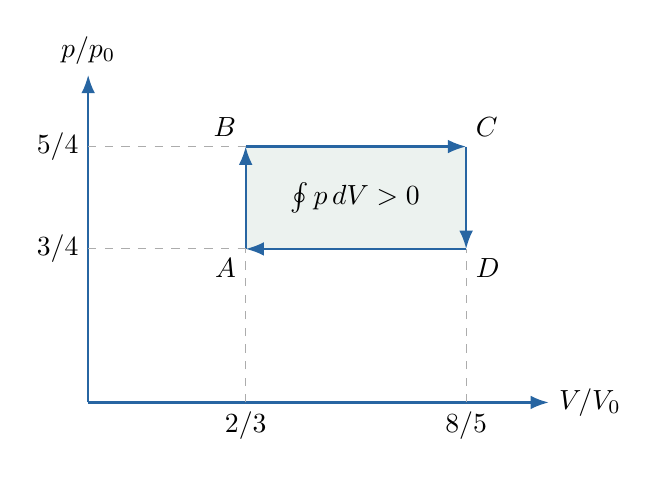
\begin{tikzpicture}[x=3cm,y=2.6cm]
 \draw[vec](0,0)--(1.95,0)node[right]{$V/V_0$};
 \draw[vec](0,0)--(0,1.6)node[above]{$p/p_0$};
 \fill[green!10](.6667,.75)rectangle(1.6,1.25);
 \draw[vec](.6667,.75)--(.6667,1.25);
 \draw[vec](.6667,1.25)--(1.6,1.25);
 \draw[vec](1.6,1.25)--(1.6,.75);
 \draw[vec](1.6,.75)--(.6667,.75);
 \draw[guide](0,.75)--(.6667,.75)(0,1.25)--(.6667,1.25)(.6667,0)--(.6667,.75)(1.6,0)--(1.6,.75);
 \node[below left]at(.6667,.75){$A$};\node[above left]at(.6667,1.25){$B$};
 \node[above right]at(1.6,1.25){$C$};\node[below right]at(1.6,.75){$D$};
 \node[left]at(0,.75){$3/4$};\node[left]at(0,1.25){$5/4$};
 \node[below]at(.6667,0){$2/3$};\node[below]at(1.6,0){$8/5$};
 \node at(1.13,1){$\oint p\,dV>0$};
\end{tikzpicture}
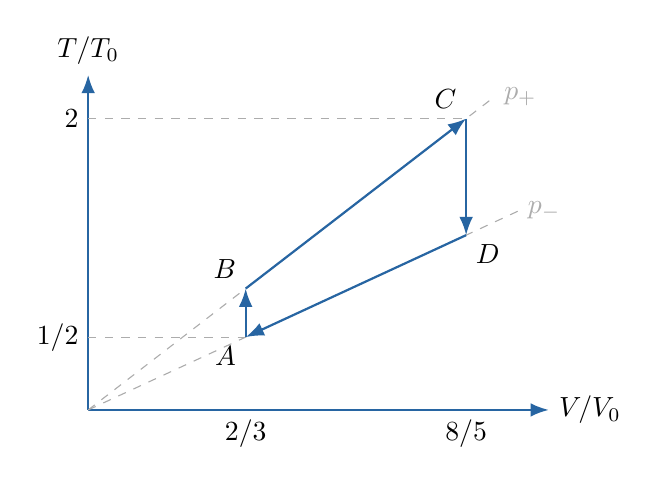
\begin{tikzpicture}[x=3cm,y=1.85cm]
 \draw[vec](0,0)--(1.95,0)node[right]{$V/V_0$};
 \draw[vec](0,0)--(0,2.3)node[above]{$T/T_0$};
 \draw[guide](0,0)--(1.72,2.15)node[right]{$p_+$};
 \draw[guide](0,0)--(1.82,1.365)node[right]{$p_-$};
 \draw[vec](.6667,.5)--(.6667,.8333);
 \draw[vec](.6667,.8333)--(1.6,2);
 \draw[vec](1.6,2)--(1.6,1.2);
 \draw[vec](1.6,1.2)--(.6667,.5);
 \node[below left]at(.6667,.5){$A$};\node[above left]at(.6667,.8333){$B$};
 \node[above left]at(1.6,2){$C$};\node[below right]at(1.6,1.2){$D$};
 \node[below]at(.6667,0){$2/3$};\node[below]at(1.6,0){$8/5$};
 \draw[guide](0,.5)--(.6667,.5)(0,2)--(1.6,2);
 \node[left]at(0,.5){$1/2$};\node[left]at(0,2){$2$};
\end{tikzpicture}
\end{document}
